% 
% Modelo de artigo científico para a Faculdade de Tecnlogia SENAI "Mariano Ferraz"
%
% Curso de Pós-Graduação em Internet das Coisas
%
% e-mail dos integrantes do grupo:
% Rafael Gomes de Paula: rpaula@senaisp.edu.br


\documentclass[
	% -- opções da classe memoir --
	article,			% indica que é um artigo acadêmico
	12pt,				% tamanho da fonte
	oneside,			% para impressão apenas no verso. Oposto a twoside
	a4paper,			% tamanho do papel. 
	% -- opções do pacote babel --
	english,			% idioma adicional para hifenização
	brazil,				% o último idioma é o principal do documento
	sumario=tradicional
	]{abntex2}


% ---
% PACOTES
% ---

% ---
% Pacotes fundamentais 
% ---
\usepackage{lmodern}			% Usa a fonte Latin Modern
\usepackage[T1]{fontenc}		% Selecao de codigos de fonte.
\usepackage[utf8]{inputenc}		% Codificacao do documento (conversão automática dos acentos)
\usepackage{nomencl} 			% Lista de simbolos
\usepackage{color}				% Controle das cores
\usepackage{graphicx}			% Inclusão de gráficos
\usepackage{microtype} 			% Para melhorias de justificação
\usepackage{float}				% Para ajuste na posição de figuras e tabelas
\usepackage{cite}				% Para ajuste na posição de figuras e tabelas
\usepackage{listings}			% Para reconhecimento da Linguagem de programação
\usepackage{xcolor}				% Controle das cores

% ---
		
% ---
% Pacotes adicionais, usados apenas no âmbito do Modelo Canônico do abnteX2
% ---
\usepackage{lipsum}				% para geração de dummy text
% ---
		
% ---
% Pacotes de citações
% ---
\usepackage[brazilian,hyperpageref]{backref}	 % Paginas com as citações na bibl
\usepackage[alf]{abntex2cite}	% Citações padrão ABNT
% ---
 %%%%%%%%%%%%%%%%%%%%%%%%%%%%%%%%%%%%%%%%%%%%%%%%%%%%%%%%%%%%%%%%%%%%%%%%%%%%%%%% 
%%% ~ Arduino Language - Arduino IDE Colors ~                                  %%%
%%%                                                                            %%%
%%% Kyle Rocha-Brownell | 10/2/2017 | No Licence                               %%%
%%% -------------------------------------------------------------------------- %%%
%%%                                                                            %%%
%%% Place this file in your working directory (next to the latex file you're   %%%
%%% working on).  To add it to your project, place:                            %%%
%%%     %%%%%%%%%%%%%%%%%%%%%%%%%%%%%%%%%%%%%%%%%%%%%%%%%%%%%%%%%%%%%%%%%%%%%%%%%%%%%%%% 
%%% ~ Arduino Language - Arduino IDE Colors ~                                  %%%
%%%                                                                            %%%
%%% Kyle Rocha-Brownell | 10/2/2017 | No Licence                               %%%
%%% -------------------------------------------------------------------------- %%%
%%%                                                                            %%%
%%% Place this file in your working directory (next to the latex file you're   %%%
%%% working on).  To add it to your project, place:                            %%%
%%%     %%%%%%%%%%%%%%%%%%%%%%%%%%%%%%%%%%%%%%%%%%%%%%%%%%%%%%%%%%%%%%%%%%%%%%%%%%%%%%%% 
%%% ~ Arduino Language - Arduino IDE Colors ~                                  %%%
%%%                                                                            %%%
%%% Kyle Rocha-Brownell | 10/2/2017 | No Licence                               %%%
%%% -------------------------------------------------------------------------- %%%
%%%                                                                            %%%
%%% Place this file in your working directory (next to the latex file you're   %%%
%%% working on).  To add it to your project, place:                            %%%
%%%    \input{arduinoLanguage.tex}                                             %%%
%%% somewhere before \begin{document} in your latex file.                      %%%
%%%                                                                            %%%
%%% In your document, place your arduino code between:                         %%%
%%%   \begin{lstlisting}[language=Arduino]                                     %%%
%%% and:                                                                       %%%
%%%   \end{lstlisting}                                                         %%%
%%%                                                                            %%%
%%% Or create your own style to add non-built-in functions and variables.      %%%
%%%                                                                            %%%
 %%%%%%%%%%%%%%%%%%%%%%%%%%%%%%%%%%%%%%%%%%%%%%%%%%%%%%%%%%%%%%%%%%%%%%%%%%%%%%%% 

\usepackage{color}
\usepackage{listings}    
\usepackage{courier}

%%% Define Custom IDE Colors %%%
\definecolor{arduinoGreen}    {rgb} {0.17, 0.43, 0.01}
\definecolor{arduinoGrey}     {rgb} {0.47, 0.47, 0.33}
\definecolor{arduinoOrange}   {rgb} {0.8 , 0.4 , 0   }
\definecolor{arduinoBlue}     {rgb} {0.01, 0.61, 0.98}
\definecolor{arduinoDarkBlue} {rgb} {0.0 , 0.2 , 0.5 }

%%% Define Arduino Language %%%
\lstdefinelanguage{Arduino}{
  language=C++, % begin with default C++ settings 
%
%
  %%% Keyword Color Group 1 %%%  (called KEYWORD3 by arduino)
  keywordstyle=\color{arduinoGreen},   
  deletekeywords={  % remove all arduino keywords that might be in c++
                break, case, override, final, continue, default, do, else, for, 
                if, return, goto, switch, throw, try, while, setup, loop, export, 
                not, or, and, xor, include, define, elif, else, error, if, ifdef, 
                ifndef, pragma, warning,
                HIGH, LOW, INPUT, INPUT_PULLUP, OUTPUT, DEC, BIN, HEX, OCT, PI, 
                HALF_PI, TWO_PI, LSBFIRST, MSBFIRST, CHANGE, FALLING, RISING, 
                DEFAULT, EXTERNAL, INTERNAL, INTERNAL1V1, INTERNAL2V56, LED_BUILTIN, 
                LED_BUILTIN_RX, LED_BUILTIN_TX, DIGITAL_MESSAGE, FIRMATA_STRING, 
                ANALOG_MESSAGE, REPORT_DIGITAL, REPORT_ANALOG, SET_PIN_MODE, 
                SYSTEM_RESET, SYSEX_START, auto, int8_t, int16_t, int32_t, int64_t, 
                uint8_t, uint16_t, uint32_t, uint64_t, char16_t, char32_t, operator, 
                enum, delete, bool, boolean, byte, char, const, false, float, double, 
                null, NULL, int, long, new, private, protected, public, short, 
                signed, static, volatile, String, void, true, unsigned, word, array, 
                sizeof, dynamic_cast, typedef, const_cast, struct, static_cast, union, 
                friend, extern, class, reinterpret_cast, register, explicit, inline, 
                _Bool, complex, _Complex, _Imaginary, atomic_bool, atomic_char, 
                atomic_schar, atomic_uchar, atomic_short, atomic_ushort, atomic_int, 
                atomic_uint, atomic_long, atomic_ulong, atomic_llong, atomic_ullong, 
                virtual, PROGMEM,
                Serial, Serial1, Serial2, Serial3, SerialUSB, Keyboard, Mouse,
                abs, acos, asin, atan, atan2, ceil, constrain, cos, degrees, exp, 
                floor, log, map, max, min, radians, random, randomSeed, round, sin, 
                sq, sqrt, tan, pow, bitRead, bitWrite, bitSet, bitClear, bit, 
                highByte, lowByte, analogReference, analogRead, 
                analogReadResolution, analogWrite, analogWriteResolution, 
                attachInterrupt, detachInterrupt, digitalPinToInterrupt, delay, 
                delayMicroseconds, digitalWrite, digitalRead, interrupts, millis, 
                micros, noInterrupts, noTone, pinMode, pulseIn, pulseInLong, shiftIn, 
                shiftOut, tone, yield, Stream, begin, end, peek, read, print, 
                println, available, availableForWrite, flush, setTimeout, find, 
                findUntil, parseInt, parseFloat, readBytes, readBytesUntil, readString, 
                readStringUntil, trim, toUpperCase, toLowerCase, charAt, compareTo, 
                concat, endsWith, startsWith, equals, equalsIgnoreCase, getBytes, 
                indexOf, lastIndexOf, length, replace, setCharAt, substring, 
                toCharArray, toInt, press, release, releaseAll, accept, click, move, 
                isPressed, isAlphaNumeric, isAlpha, isAscii, isWhitespace, isControl, 
                isDigit, isGraph, isLowerCase, isPrintable, isPunct, isSpace, 
                isUpperCase, isHexadecimalDigit, 
                }, 
  morekeywords={   % add arduino structures to group 1
                break, case, override, final, continue, default, do, else, for, 
                if, return, goto, switch, throw, try, while, setup, loop, export, 
                not, or, and, xor, include, define, elif, else, error, if, ifdef, 
                ifndef, pragma, warning,
                }, 
% 
%
  %%% Keyword Color Group 2 %%%  (called LITERAL1 by arduino)
  keywordstyle=[2]\color{arduinoBlue},   
  keywords=[2]{   % add variables and dataTypes as 2nd group  
                HIGH, LOW, INPUT, INPUT_PULLUP, OUTPUT, DEC, BIN, HEX, OCT, PI, 
                HALF_PI, TWO_PI, LSBFIRST, MSBFIRST, CHANGE, FALLING, RISING, 
                DEFAULT, EXTERNAL, INTERNAL, INTERNAL1V1, INTERNAL2V56, LED_BUILTIN, 
                LED_BUILTIN_RX, LED_BUILTIN_TX, DIGITAL_MESSAGE, FIRMATA_STRING, 
                ANALOG_MESSAGE, REPORT_DIGITAL, REPORT_ANALOG, SET_PIN_MODE, 
                SYSTEM_RESET, SYSEX_START, auto, int8_t, int16_t, int32_t, int64_t, 
                uint8_t, uint16_t, uint32_t, uint64_t, char16_t, char32_t, operator, 
                enum, delete, bool, boolean, byte, char, const, false, float, double, 
                null, NULL, int, long, new, private, protected, public, short, 
                signed, static, volatile, String, void, true, unsigned, word, array, 
                sizeof, dynamic_cast, typedef, const_cast, struct, static_cast, union, 
                friend, extern, class, reinterpret_cast, register, explicit, inline, 
                _Bool, complex, _Complex, _Imaginary, atomic_bool, atomic_char, 
                atomic_schar, atomic_uchar, atomic_short, atomic_ushort, atomic_int, 
                atomic_uint, atomic_long, atomic_ulong, atomic_llong, atomic_ullong, 
                virtual, PROGMEM,
                },  
% 
%
  %%% Keyword Color Group 3 %%%  (called KEYWORD1 by arduino)
  keywordstyle=[3]\bfseries\color{arduinoOrange},
  keywords=[3]{  % add built-in functions as a 3rd group
                Serial, Serial1, Serial2, Serial3, SerialUSB, Keyboard, Mouse,
                },      
%
%
  %%% Keyword Color Group 4 %%%  (called KEYWORD2 by arduino)
  keywordstyle=[4]\color{arduinoOrange},
  keywords=[4]{  % add more built-in functions as a 4th group
                abs, acos, asin, atan, atan2, ceil, constrain, cos, degrees, exp, 
                floor, log, map, max, min, radians, random, randomSeed, round, sin, 
                sq, sqrt, tan, pow, bitRead, bitWrite, bitSet, bitClear, bit, 
                highByte, lowByte, analogReference, analogRead, 
                analogReadResolution, analogWrite, analogWriteResolution, 
                attachInterrupt, detachInterrupt, digitalPinToInterrupt, delay, 
                delayMicroseconds, digitalWrite, digitalRead, interrupts, millis, 
                micros, noInterrupts, noTone, pinMode, pulseIn, pulseInLong, shiftIn, 
                shiftOut, tone, yield, Stream, begin, end, peek, read, print, 
                println, available, availableForWrite, flush, setTimeout, find, 
                findUntil, parseInt, parseFloat, readBytes, readBytesUntil, readString, 
                readStringUntil, trim, toUpperCase, toLowerCase, charAt, compareTo, 
                concat, endsWith, startsWith, equals, equalsIgnoreCase, getBytes, 
                indexOf, lastIndexOf, length, replace, setCharAt, substring, 
                toCharArray, toInt, press, release, releaseAll, accept, click, move, 
                isPressed, isAlphaNumeric, isAlpha, isAscii, isWhitespace, isControl, 
                isDigit, isGraph, isLowerCase, isPrintable, isPunct, isSpace, 
                isUpperCase, isHexadecimalDigit, 
                },      
%
%
  %%% Set Other Colors %%%
  stringstyle=\color{arduinoDarkBlue},    
  commentstyle=\color{arduinoGrey},    
%          
%   
  %%%% Line Numbering %%%%
  numbers=left,                    
  numbersep=5pt,                   
  numberstyle=\color{arduinoGrey},    
  %stepnumber=2,                      % show every 2 line numbers
%
%
  %%%% Code Box Style %%%%
  breaklines=true,                    % wordwrapping
  tabsize=2,         
  basicstyle=\ttfamily  
}
                                             %%%
%%% somewhere before \begin{document} in your latex file.                      %%%
%%%                                                                            %%%
%%% In your document, place your arduino code between:                         %%%
%%%   \begin{lstlisting}[language=Arduino]                                     %%%
%%% and:                                                                       %%%
%%%   \end{lstlisting}                                                         %%%
%%%                                                                            %%%
%%% Or create your own style to add non-built-in functions and variables.      %%%
%%%                                                                            %%%
 %%%%%%%%%%%%%%%%%%%%%%%%%%%%%%%%%%%%%%%%%%%%%%%%%%%%%%%%%%%%%%%%%%%%%%%%%%%%%%%% 

\usepackage{color}
\usepackage{listings}    
\usepackage{courier}

%%% Define Custom IDE Colors %%%
\definecolor{arduinoGreen}    {rgb} {0.17, 0.43, 0.01}
\definecolor{arduinoGrey}     {rgb} {0.47, 0.47, 0.33}
\definecolor{arduinoOrange}   {rgb} {0.8 , 0.4 , 0   }
\definecolor{arduinoBlue}     {rgb} {0.01, 0.61, 0.98}
\definecolor{arduinoDarkBlue} {rgb} {0.0 , 0.2 , 0.5 }

%%% Define Arduino Language %%%
\lstdefinelanguage{Arduino}{
  language=C++, % begin with default C++ settings 
%
%
  %%% Keyword Color Group 1 %%%  (called KEYWORD3 by arduino)
  keywordstyle=\color{arduinoGreen},   
  deletekeywords={  % remove all arduino keywords that might be in c++
                break, case, override, final, continue, default, do, else, for, 
                if, return, goto, switch, throw, try, while, setup, loop, export, 
                not, or, and, xor, include, define, elif, else, error, if, ifdef, 
                ifndef, pragma, warning,
                HIGH, LOW, INPUT, INPUT_PULLUP, OUTPUT, DEC, BIN, HEX, OCT, PI, 
                HALF_PI, TWO_PI, LSBFIRST, MSBFIRST, CHANGE, FALLING, RISING, 
                DEFAULT, EXTERNAL, INTERNAL, INTERNAL1V1, INTERNAL2V56, LED_BUILTIN, 
                LED_BUILTIN_RX, LED_BUILTIN_TX, DIGITAL_MESSAGE, FIRMATA_STRING, 
                ANALOG_MESSAGE, REPORT_DIGITAL, REPORT_ANALOG, SET_PIN_MODE, 
                SYSTEM_RESET, SYSEX_START, auto, int8_t, int16_t, int32_t, int64_t, 
                uint8_t, uint16_t, uint32_t, uint64_t, char16_t, char32_t, operator, 
                enum, delete, bool, boolean, byte, char, const, false, float, double, 
                null, NULL, int, long, new, private, protected, public, short, 
                signed, static, volatile, String, void, true, unsigned, word, array, 
                sizeof, dynamic_cast, typedef, const_cast, struct, static_cast, union, 
                friend, extern, class, reinterpret_cast, register, explicit, inline, 
                _Bool, complex, _Complex, _Imaginary, atomic_bool, atomic_char, 
                atomic_schar, atomic_uchar, atomic_short, atomic_ushort, atomic_int, 
                atomic_uint, atomic_long, atomic_ulong, atomic_llong, atomic_ullong, 
                virtual, PROGMEM,
                Serial, Serial1, Serial2, Serial3, SerialUSB, Keyboard, Mouse,
                abs, acos, asin, atan, atan2, ceil, constrain, cos, degrees, exp, 
                floor, log, map, max, min, radians, random, randomSeed, round, sin, 
                sq, sqrt, tan, pow, bitRead, bitWrite, bitSet, bitClear, bit, 
                highByte, lowByte, analogReference, analogRead, 
                analogReadResolution, analogWrite, analogWriteResolution, 
                attachInterrupt, detachInterrupt, digitalPinToInterrupt, delay, 
                delayMicroseconds, digitalWrite, digitalRead, interrupts, millis, 
                micros, noInterrupts, noTone, pinMode, pulseIn, pulseInLong, shiftIn, 
                shiftOut, tone, yield, Stream, begin, end, peek, read, print, 
                println, available, availableForWrite, flush, setTimeout, find, 
                findUntil, parseInt, parseFloat, readBytes, readBytesUntil, readString, 
                readStringUntil, trim, toUpperCase, toLowerCase, charAt, compareTo, 
                concat, endsWith, startsWith, equals, equalsIgnoreCase, getBytes, 
                indexOf, lastIndexOf, length, replace, setCharAt, substring, 
                toCharArray, toInt, press, release, releaseAll, accept, click, move, 
                isPressed, isAlphaNumeric, isAlpha, isAscii, isWhitespace, isControl, 
                isDigit, isGraph, isLowerCase, isPrintable, isPunct, isSpace, 
                isUpperCase, isHexadecimalDigit, 
                }, 
  morekeywords={   % add arduino structures to group 1
                break, case, override, final, continue, default, do, else, for, 
                if, return, goto, switch, throw, try, while, setup, loop, export, 
                not, or, and, xor, include, define, elif, else, error, if, ifdef, 
                ifndef, pragma, warning,
                }, 
% 
%
  %%% Keyword Color Group 2 %%%  (called LITERAL1 by arduino)
  keywordstyle=[2]\color{arduinoBlue},   
  keywords=[2]{   % add variables and dataTypes as 2nd group  
                HIGH, LOW, INPUT, INPUT_PULLUP, OUTPUT, DEC, BIN, HEX, OCT, PI, 
                HALF_PI, TWO_PI, LSBFIRST, MSBFIRST, CHANGE, FALLING, RISING, 
                DEFAULT, EXTERNAL, INTERNAL, INTERNAL1V1, INTERNAL2V56, LED_BUILTIN, 
                LED_BUILTIN_RX, LED_BUILTIN_TX, DIGITAL_MESSAGE, FIRMATA_STRING, 
                ANALOG_MESSAGE, REPORT_DIGITAL, REPORT_ANALOG, SET_PIN_MODE, 
                SYSTEM_RESET, SYSEX_START, auto, int8_t, int16_t, int32_t, int64_t, 
                uint8_t, uint16_t, uint32_t, uint64_t, char16_t, char32_t, operator, 
                enum, delete, bool, boolean, byte, char, const, false, float, double, 
                null, NULL, int, long, new, private, protected, public, short, 
                signed, static, volatile, String, void, true, unsigned, word, array, 
                sizeof, dynamic_cast, typedef, const_cast, struct, static_cast, union, 
                friend, extern, class, reinterpret_cast, register, explicit, inline, 
                _Bool, complex, _Complex, _Imaginary, atomic_bool, atomic_char, 
                atomic_schar, atomic_uchar, atomic_short, atomic_ushort, atomic_int, 
                atomic_uint, atomic_long, atomic_ulong, atomic_llong, atomic_ullong, 
                virtual, PROGMEM,
                },  
% 
%
  %%% Keyword Color Group 3 %%%  (called KEYWORD1 by arduino)
  keywordstyle=[3]\bfseries\color{arduinoOrange},
  keywords=[3]{  % add built-in functions as a 3rd group
                Serial, Serial1, Serial2, Serial3, SerialUSB, Keyboard, Mouse,
                },      
%
%
  %%% Keyword Color Group 4 %%%  (called KEYWORD2 by arduino)
  keywordstyle=[4]\color{arduinoOrange},
  keywords=[4]{  % add more built-in functions as a 4th group
                abs, acos, asin, atan, atan2, ceil, constrain, cos, degrees, exp, 
                floor, log, map, max, min, radians, random, randomSeed, round, sin, 
                sq, sqrt, tan, pow, bitRead, bitWrite, bitSet, bitClear, bit, 
                highByte, lowByte, analogReference, analogRead, 
                analogReadResolution, analogWrite, analogWriteResolution, 
                attachInterrupt, detachInterrupt, digitalPinToInterrupt, delay, 
                delayMicroseconds, digitalWrite, digitalRead, interrupts, millis, 
                micros, noInterrupts, noTone, pinMode, pulseIn, pulseInLong, shiftIn, 
                shiftOut, tone, yield, Stream, begin, end, peek, read, print, 
                println, available, availableForWrite, flush, setTimeout, find, 
                findUntil, parseInt, parseFloat, readBytes, readBytesUntil, readString, 
                readStringUntil, trim, toUpperCase, toLowerCase, charAt, compareTo, 
                concat, endsWith, startsWith, equals, equalsIgnoreCase, getBytes, 
                indexOf, lastIndexOf, length, replace, setCharAt, substring, 
                toCharArray, toInt, press, release, releaseAll, accept, click, move, 
                isPressed, isAlphaNumeric, isAlpha, isAscii, isWhitespace, isControl, 
                isDigit, isGraph, isLowerCase, isPrintable, isPunct, isSpace, 
                isUpperCase, isHexadecimalDigit, 
                },      
%
%
  %%% Set Other Colors %%%
  stringstyle=\color{arduinoDarkBlue},    
  commentstyle=\color{arduinoGrey},    
%          
%   
  %%%% Line Numbering %%%%
  numbers=left,                    
  numbersep=5pt,                   
  numberstyle=\color{arduinoGrey},    
  %stepnumber=2,                      % show every 2 line numbers
%
%
  %%%% Code Box Style %%%%
  breaklines=true,                    % wordwrapping
  tabsize=2,         
  basicstyle=\ttfamily  
}
                                             %%%
%%% somewhere before \begin{document} in your latex file.                      %%%
%%%                                                                            %%%
%%% In your document, place your arduino code between:                         %%%
%%%   \begin{lstlisting}[language=Arduino]                                     %%%
%%% and:                                                                       %%%
%%%   \end{lstlisting}                                                         %%%
%%%                                                                            %%%
%%% Or create your own style to add non-built-in functions and variables.      %%%
%%%                                                                            %%%
 %%%%%%%%%%%%%%%%%%%%%%%%%%%%%%%%%%%%%%%%%%%%%%%%%%%%%%%%%%%%%%%%%%%%%%%%%%%%%%%% 

\usepackage{color}
\usepackage{listings}    
\usepackage{courier}

%%% Define Custom IDE Colors %%%
\definecolor{arduinoGreen}    {rgb} {0.17, 0.43, 0.01}
\definecolor{arduinoGrey}     {rgb} {0.47, 0.47, 0.33}
\definecolor{arduinoOrange}   {rgb} {0.8 , 0.4 , 0   }
\definecolor{arduinoBlue}     {rgb} {0.01, 0.61, 0.98}
\definecolor{arduinoDarkBlue} {rgb} {0.0 , 0.2 , 0.5 }

%%% Define Arduino Language %%%
\lstdefinelanguage{Arduino}{
  language=C++, % begin with default C++ settings 
%
%
  %%% Keyword Color Group 1 %%%  (called KEYWORD3 by arduino)
  keywordstyle=\color{arduinoGreen},   
  deletekeywords={  % remove all arduino keywords that might be in c++
                break, case, override, final, continue, default, do, else, for, 
                if, return, goto, switch, throw, try, while, setup, loop, export, 
                not, or, and, xor, include, define, elif, else, error, if, ifdef, 
                ifndef, pragma, warning,
                HIGH, LOW, INPUT, INPUT_PULLUP, OUTPUT, DEC, BIN, HEX, OCT, PI, 
                HALF_PI, TWO_PI, LSBFIRST, MSBFIRST, CHANGE, FALLING, RISING, 
                DEFAULT, EXTERNAL, INTERNAL, INTERNAL1V1, INTERNAL2V56, LED_BUILTIN, 
                LED_BUILTIN_RX, LED_BUILTIN_TX, DIGITAL_MESSAGE, FIRMATA_STRING, 
                ANALOG_MESSAGE, REPORT_DIGITAL, REPORT_ANALOG, SET_PIN_MODE, 
                SYSTEM_RESET, SYSEX_START, auto, int8_t, int16_t, int32_t, int64_t, 
                uint8_t, uint16_t, uint32_t, uint64_t, char16_t, char32_t, operator, 
                enum, delete, bool, boolean, byte, char, const, false, float, double, 
                null, NULL, int, long, new, private, protected, public, short, 
                signed, static, volatile, String, void, true, unsigned, word, array, 
                sizeof, dynamic_cast, typedef, const_cast, struct, static_cast, union, 
                friend, extern, class, reinterpret_cast, register, explicit, inline, 
                _Bool, complex, _Complex, _Imaginary, atomic_bool, atomic_char, 
                atomic_schar, atomic_uchar, atomic_short, atomic_ushort, atomic_int, 
                atomic_uint, atomic_long, atomic_ulong, atomic_llong, atomic_ullong, 
                virtual, PROGMEM,
                Serial, Serial1, Serial2, Serial3, SerialUSB, Keyboard, Mouse,
                abs, acos, asin, atan, atan2, ceil, constrain, cos, degrees, exp, 
                floor, log, map, max, min, radians, random, randomSeed, round, sin, 
                sq, sqrt, tan, pow, bitRead, bitWrite, bitSet, bitClear, bit, 
                highByte, lowByte, analogReference, analogRead, 
                analogReadResolution, analogWrite, analogWriteResolution, 
                attachInterrupt, detachInterrupt, digitalPinToInterrupt, delay, 
                delayMicroseconds, digitalWrite, digitalRead, interrupts, millis, 
                micros, noInterrupts, noTone, pinMode, pulseIn, pulseInLong, shiftIn, 
                shiftOut, tone, yield, Stream, begin, end, peek, read, print, 
                println, available, availableForWrite, flush, setTimeout, find, 
                findUntil, parseInt, parseFloat, readBytes, readBytesUntil, readString, 
                readStringUntil, trim, toUpperCase, toLowerCase, charAt, compareTo, 
                concat, endsWith, startsWith, equals, equalsIgnoreCase, getBytes, 
                indexOf, lastIndexOf, length, replace, setCharAt, substring, 
                toCharArray, toInt, press, release, releaseAll, accept, click, move, 
                isPressed, isAlphaNumeric, isAlpha, isAscii, isWhitespace, isControl, 
                isDigit, isGraph, isLowerCase, isPrintable, isPunct, isSpace, 
                isUpperCase, isHexadecimalDigit, 
                }, 
  morekeywords={   % add arduino structures to group 1
                break, case, override, final, continue, default, do, else, for, 
                if, return, goto, switch, throw, try, while, setup, loop, export, 
                not, or, and, xor, include, define, elif, else, error, if, ifdef, 
                ifndef, pragma, warning,
                }, 
% 
%
  %%% Keyword Color Group 2 %%%  (called LITERAL1 by arduino)
  keywordstyle=[2]\color{arduinoBlue},   
  keywords=[2]{   % add variables and dataTypes as 2nd group  
                HIGH, LOW, INPUT, INPUT_PULLUP, OUTPUT, DEC, BIN, HEX, OCT, PI, 
                HALF_PI, TWO_PI, LSBFIRST, MSBFIRST, CHANGE, FALLING, RISING, 
                DEFAULT, EXTERNAL, INTERNAL, INTERNAL1V1, INTERNAL2V56, LED_BUILTIN, 
                LED_BUILTIN_RX, LED_BUILTIN_TX, DIGITAL_MESSAGE, FIRMATA_STRING, 
                ANALOG_MESSAGE, REPORT_DIGITAL, REPORT_ANALOG, SET_PIN_MODE, 
                SYSTEM_RESET, SYSEX_START, auto, int8_t, int16_t, int32_t, int64_t, 
                uint8_t, uint16_t, uint32_t, uint64_t, char16_t, char32_t, operator, 
                enum, delete, bool, boolean, byte, char, const, false, float, double, 
                null, NULL, int, long, new, private, protected, public, short, 
                signed, static, volatile, String, void, true, unsigned, word, array, 
                sizeof, dynamic_cast, typedef, const_cast, struct, static_cast, union, 
                friend, extern, class, reinterpret_cast, register, explicit, inline, 
                _Bool, complex, _Complex, _Imaginary, atomic_bool, atomic_char, 
                atomic_schar, atomic_uchar, atomic_short, atomic_ushort, atomic_int, 
                atomic_uint, atomic_long, atomic_ulong, atomic_llong, atomic_ullong, 
                virtual, PROGMEM,
                },  
% 
%
  %%% Keyword Color Group 3 %%%  (called KEYWORD1 by arduino)
  keywordstyle=[3]\bfseries\color{arduinoOrange},
  keywords=[3]{  % add built-in functions as a 3rd group
                Serial, Serial1, Serial2, Serial3, SerialUSB, Keyboard, Mouse,
                },      
%
%
  %%% Keyword Color Group 4 %%%  (called KEYWORD2 by arduino)
  keywordstyle=[4]\color{arduinoOrange},
  keywords=[4]{  % add more built-in functions as a 4th group
                abs, acos, asin, atan, atan2, ceil, constrain, cos, degrees, exp, 
                floor, log, map, max, min, radians, random, randomSeed, round, sin, 
                sq, sqrt, tan, pow, bitRead, bitWrite, bitSet, bitClear, bit, 
                highByte, lowByte, analogReference, analogRead, 
                analogReadResolution, analogWrite, analogWriteResolution, 
                attachInterrupt, detachInterrupt, digitalPinToInterrupt, delay, 
                delayMicroseconds, digitalWrite, digitalRead, interrupts, millis, 
                micros, noInterrupts, noTone, pinMode, pulseIn, pulseInLong, shiftIn, 
                shiftOut, tone, yield, Stream, begin, end, peek, read, print, 
                println, available, availableForWrite, flush, setTimeout, find, 
                findUntil, parseInt, parseFloat, readBytes, readBytesUntil, readString, 
                readStringUntil, trim, toUpperCase, toLowerCase, charAt, compareTo, 
                concat, endsWith, startsWith, equals, equalsIgnoreCase, getBytes, 
                indexOf, lastIndexOf, length, replace, setCharAt, substring, 
                toCharArray, toInt, press, release, releaseAll, accept, click, move, 
                isPressed, isAlphaNumeric, isAlpha, isAscii, isWhitespace, isControl, 
                isDigit, isGraph, isLowerCase, isPrintable, isPunct, isSpace, 
                isUpperCase, isHexadecimalDigit, 
                },      
%
%
  %%% Set Other Colors %%%
  stringstyle=\color{arduinoDarkBlue},    
  commentstyle=\color{arduinoGrey},    
%          
%   
  %%%% Line Numbering %%%%
  numbers=left,                    
  numbersep=5pt,                   
  numberstyle=\color{arduinoGrey},    
  %stepnumber=2,                      % show every 2 line numbers
%
%
  %%%% Code Box Style %%%%
  breaklines=true,                    % wordwrapping
  tabsize=2,         
  basicstyle=\ttfamily  
}
    % adds the arduino language listing

% ---
% Pacotes de citações
% ---
\graphicspath{ {./images/} }
% ---

% ---
% Configurações do pacote backref
% ---
% Usado sem a opção hyperpageref de backref
\renewcommand{\backrefpagesname}{Citado na(s) página(s):~}
% Texto padrão antes do número das páginas
\renewcommand{\backref}{}
% Define os textos da citação
\renewcommand*{\backrefalt}[4]{
	\ifcase #1 %
		Nenhuma citação no texto.%
	\or
		Citado na página #2.%
	\else
		Citado #1 vezes nas páginas #2.%
	\fi}%
% ---

% ---
% Informações de dados para CAPA e FOLHA DE ROSTO
% ---
\titulo{Projeto para localização de dispositivos bluetooth BLE indoor}
\autor{Josimar de Andrade Silva, \and Rafael Gomes de Paula,\and Wanderson Thiago da Silva Pagani}
\local{Brasil}
\data{24/03/2020} 
% ---

%% Define an Arduino style fore use later %%
\lstdefinestyle{myArduino}{
  language=Arduino,
  %% Add other words needing highlighting below %%
  morekeywords=[1]{},                  % [1] -> dark green
  morekeywords=[2]{FILE_WRITE},        % [2] -> light blue
  morekeywords=[3]{SD, File},          % [3] -> bold orange
  morekeywords=[4]{open, exists},      % [4] -> orange
  %% The lines below add a nifty box around the code %%
  frame=shadowbox,
  rulesepcolor=\color{arduinoBlue},
}
% ---
% ---
% Alterando o aspecto da cor azul
% ---
\definecolor{blue}{RGB}{41,5,195}
% ---

% ---
% Informações do PDF
% ---
\makeatletter
\hypersetup{
     	%pagebackref=true,
		pdftitle={\@title}, 
		pdfauthor={\@author},
    	pdfsubject={Projeto Localização Indoor},
	    pdfcreator={LaTeX with abnTeX2},
		pdfkeywords={abnt}{latex}{abntex}{abntex2}{artigo científico}, 
		colorlinks=true,       		% false: boxed links; true: colored links
    	linkcolor=blue,          	% color of internal links
    	citecolor=blue,        		% color of links to bibliography
    	filecolor=magenta,      		% color of file links
		urlcolor=blue,
		bookmarksdepth=4
}
\makeatother
% --- 

% ---
% Compila o índice
% ---
\makeindex
% ---

% ---
% Altera as margens padrões
% ---
\setlrmarginsandblock{2cm}{2cm}{*}
\setulmarginsandblock{2cm}{2cm}{*}
\checkandfixthelayout
% ---

% --- 
% Espaçamentos entre linhas e parágrafos 
% --- 

% O tamanho do parágrafo é dado por:
\setlength{\parindent}{.5cm}

% Controle do espaçamento entre um parágrafo e outro:
\setlength{\parskip}{0.2cm}  % tente também \onelineskip

% Espaçamento simples
\SingleSpacing
% ---

% --- 
% Cabeçalho 
% --- 
\makepagestyle{meuestilo}
  \makeoddhead{meuestilo} %%pagina ímpar ou com oneside
     {Faculdade de Tecnologia SENAI "Mariano Ferraz"}
     %{Vol. 1,  n\textsuperscript{o} 1 (2017)}
     {}
     {IoT - SSIR,  pág. \thepage}
% ---

% ---
% Margem para resumo, palavras-chave, abstract e keywords
% ---
\def\changemargin#1#2{\list{}{\rightmargin#2\leftmargin#1}\item[]}
\let\endchangemargin=\endlist 
% ----

% ---
% Início do documento
% ---
\begin{document}

% ----------------------------------------------------------
% ELEMENTOS TEXTUAIS
% ----------------------------------------------------------
\textual

% Aplica o cabeçalho em todas as páginas, excetuando-se a primeira
\pagestyle{meuestilo}

% Retira espaço extra obsoleto entre as frases.
\frenchspacing 

% Página de titulo
\maketitle

% Aplica cabeçalho na primeira página
\thispagestyle{meuestilo}
% ---

% -----------------------------------------------------------
% Resumo em português
% -----------------------------------------------------------
\begin{changemargin}{1cm}{1cm} 
 \textbf{Resumo} – A proposta do projeto é criar um sistema de localizaçao em tempo real de dispositivos bluetooth dentro de um local fechado.
 O hardware consiste na criação de um dispositivo utilizando o ESP32, capaz de localizar outros dispositivos bluetooth, como IBeacons, através da triangulação destes dispositivos que denominamos "estações de rastreamento". 
 As estações disponibilizaram as informações dos dispositivos encontrados através da internet, utilizando o protocolo MQTT e a plataforma Node-Red.
 O Software consiste em um website, construído utilizando Node.js como servidor aplicacional, capaz de se conectar ao Node-Red e fazer a interpretação dos dados.
 A plataforma é responsável por receber os dados e determinar qual é o dispositivo mais proximo dentro do raio da triangulação das estações.
 \vspace{\onelineskip}
 
 \noindent
 \textbf{Palavras-chave} – IoT; Internet das Coisas; Comunicação; Localização; Sinal; Rádio Frequência; Alarmes; Indoor 
\end{changemargin}
% ---

% -----------------------------------------------------------
% Resumo em inglês
% -----------------------------------------------------------

\begin{changemargin}{1cm}{1cm} 
\textbf{Abstract} – The project proposal is to create a real-time location system for bluetooth devices within an enclosed location. The hardware consists of creating a device using ESP32, capable of locating other bluetooth devices, such as IBeacons, through the triangulation of these devices that we call "tracking stations". The stations made available the information of the devices found through the internet, using the MQTT protocol and the Node-Red platform. The Software consists of a website, built using Node.js as an application server, capable of connecting to Node-Red and interpreting the data. The platform is responsible for receiving the data and determining which is the closest device within the radius of the triangulation of the stations
\vspace{\onelineskip}
	
\noindent
\textbf{Keywords} – IoT; Internet of Things; Comunication; Location; Signal; Radio Frequency; Alarm; Indoor 
\end{changemargin}
   
% ---

% ----------------------------------------------------------
% Introdução
% ----------------------------------------------------------
\section{Introdução}
\addcontentsline{toc}{section}{Introdução}

% ---
% Nota de rodapé na primeira página
% ---
%\let\thefootnote\relax\footnotetext{(A ser preenchido pelos editores)  Versão inicial submetida em DD de MM. de AAAA.   Versão final aceita em DD de MM. de AAAA.  Publicado em DD de MM. de AAA.  Digital Object Identifier \_\_\_\_\_\_\slash\_\_\_\_\_ }
\let\thefootnote\svthefootnote
% ---

De acordo com LIMA (2014) o primeiro sistema de identificação por radiofrequência (RFID) surgiu em 1937 com a invenção do primeiro radar, liderado pelo escocês Sir Robert Alexander Watson-Watt da United States Naval Research Laboratory.
Após a invenção do primeiro radar, a tecnologia RFID tem sido usada para diversos tipos de aplicação, como controle de segurança, monitoramento, controle de temperatura, rastreabilidade, entre outras diversas situações.
Segundo OMEGA (2020) os sensores sem fio utilizados em aplicações de localização são ferramentas de medição padrão equipadas com transmissores utilizados para converter sinais de instrumentos de controle de processo em uma transmissão de rádio. O sinal de rádio é interpretado por um receptor que converte o sinal sem fio em uma saída específica, tal como uma corrente analógica ou uma análise de dados feita por um software.  
LOUREIRO (2003) exemplifica que cada sensor possui características particulares que variam de acordo com o ambiente e objetivo do uso, sendo alguns desses sensores: com endereçamento, para mobilidade, limitação de energia e outros.
A pesquisa apresentada neste trabalho se refere aos sensores RFID, aplicados para simplificação de atividades humanas em locais indoor. Um exemplo disso são os sistemas de localização e cálculo de distância, que utilizam as propriedades da rádio frequência como um recurso para calcular a posição ou a longitude entre dois objetos.
O objetivo principal deste trabalho é demonstrar uma das técnicas baseada no sinal Bluetooth de Baixa Energia (BLE) mais utilizadas nos sensores de localização indoor, a Indicação de Intensidade do Sinal de Rádio (RSSI), que utiliza, respectivamente, o tempo de chegada do sinal a uma ERB (Estação Base), o ângulo de chegada do sinal em relação às Estações de Rádio Base (ERB’s) e a intensidade do sinal, para calcular a posição de um objeto.  
Este trabalho, portanto, orientar-se-á no sentido de analisar o processo de localização de pessoas em um ambiente indoor de modo a utilizar a técnica RSSI, podendo ajudar a diminuir o tempo de atuação envolvendo problemas em sistemas de missão crítica.

\section{Pesquisa Bibliográfica}
Ao desenvolver as pesquisas foi utilizado o método de revisão literária, sendo esse um método qualitativo, apoiando-se em técnicas de pesquisa de dados. Realizado pela análise de conteúdos e artigos de sites, artigos técnicos, dissertações de mestrado, pesquisas bibliográficas, manuais e normas técnicas, publicados nos períodos dos últimos 20 anos, sobre o tema em questão.
Ainda é um grande desafio para as tecnologias de localização em ambientes internos. O Sistema de Posicionamento Global (GPS), por exemplo, é uma das descobertas mais eficientes, tratando-se de tecnologias baseadas nos sensores RFID. No entanto, os metros quadrados de um ambiente indoor estão fora do alcance de seus 28 satélites (LIMA, 2001). 
Na realidade, estes ambientes não são mapeados para que um sistema de GPS possa localizá-los. Desta forma, o foco de pesquisas associadas à localização de pessoas e objetos têm se baseado na busca por tecnologias apropriadas a ambientes internos. Muitas das dificuldades estão relacionadas, já que estes locais apresentam uma estrutura que não se vê externamente, como COLEMAN e (WESTCOTT, 2009):
\begin{enumerate}
	\item Alta atenuação e difusão do sinal, devido aos inúmeros obstáculos;
	\item Mudanças temporais relacionadas à movimentação de pessoas e abertura de portas;
	\item Multipath causado pela reflexão das paredes e móveis.	
\end{enumerate}	
Por outro lado, os ambientes internos oferecem algumas facilidades, já que não sofrem interferências de fatores climáticos; podem ser facilmente mapeados e possuem melhor infraestrutura (acesso a internet e energia elétrica). Portanto, neste trabalho, o estudo da localização baseada na leitura bidirecional do RSSI será destinado a ambientes indoor.

\section{Estudo de Caso}
\subsection{Objetivo}
O objetivo do estudo de caso referente a este trabalho é demonstrar a necessidade que os data centers tem em resolver problemas de infraestrutura em um menor tempo possível e o que impacta com um problema não resolvido, influenciando na sociedade.
Para demonstrar a utilização do projeto, foi escolhido o Data Center Prodesp, considerado ambiente de missão crítica, onde em uma situação de crise na infraestrutura, o tempo de atuação dos técnicos deve ser o mais rápido possível
\subsection{Justificativa}
De acordo com ICOR (2020), existem muitos fatores de risco de paralisação nos Data Centers, como falhas naturais, humanas e de origem dos hardwares e sistemas instalados. Onde o maior percentual de causas da paralisação dos data centers são por falhas humanas. 
Devido a planta do Data Center Prodesp ser de grande escala em relação ao numero de técnicos para manter a energia elétrica constante alimentando os equipamentos de Tecnologia da Informação (TI) e equipamentos de climatização (Ar-condicionado de precisão), foi possível uma projeção para melhorar o tempo de atuação dos técnicos em um ocorrência (alarmes) com o uso de um localizador de pessoas indoor por meio da tecnologia RSSI.
Considerado que a equipe de manutenção residente do Data Center Prodesp leva em média 5 minutos para localizar uma ocorrência através de um sistema supervisório Controle de Supervisão e Aquisição de Dados (SCADA), com a ajuda do localizador esse tempo pode ser menor, de acordo com a proximidade entre o técnico atuante e o equipamento em alarme. 
\subsection{Relevância para a Sociedade}
Segundo PENSO (2020), os data centers são importantes para realizar atividades simples do cotidiano, sendo desde a Internet, que você acessa para se divertir com jogos e vídeos, até os pagamentos feitos no aplicativo do seu banco, consultas de saldo e extrato, transferências ou aplicações.

\section{Definição do Projeto}
\subsection{Topologia}
A internet das coisas (IOT) proporcionou o uso do protocolo Transporte de Telemetria do Serviço de Enfileiramento de Mensagens (MQTT) para comunicação entre os hardwares de forma harmoniosa sendo possível troca de informações entre as TAG’s, ERB’s, aplicativo para celular (APP) de alarmes, software de monitoramento e servidor em nuvem. 
Segundo Zhu (2010) a origem do protocolo MQTT surgiu no laboratório Massachusetts Institute of Technology (MIT) com a pesquisa no campo de localização e identificação usando sensores sem fio, em 1999, onde deu inicio a área de estudos da Internet das Coisas.
\begin{figure}[H]
	\begin{center}
		\caption{Topologia MQTT}
		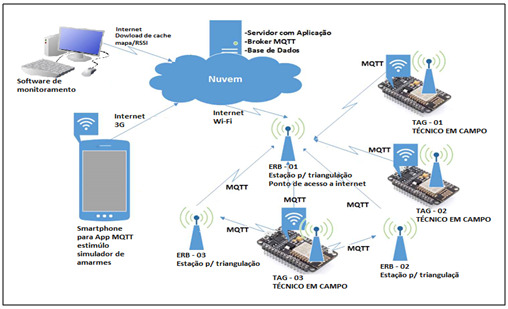
\includegraphics{image1}
		\legend{Fonte: Própria}	
	\end{center}
\end{figure}
Na figura 01 pode-se ver o fluxo de dados utilizando o protocolo MQTT para este trabalho.
O servidor com aplicação MQTT Node-RED da International Business Machines (IBM) recebe os estímulos de um APP que simula um possível alarme e equipamento instalado em um ambiente indoor. As ERB’s verificam a intensidade do sinal RFID vindas das TAG’s IBeacons, que também são informadas sobre o alarme mais próximo.
\subsection{Hardware}
A definição do hardware foi definido da seguinte forma, por placas ESP-32 para as ERBs devido a praticidade de programação e conjuntura de tecnologias RFID, por TAGs do tipo beacon paraos localizadores devido a facilidade de pessoas portarem no bolso e a tecnologia Bluetooth de Baixa Energia (BLE).
	\begin{figure}[H]
		\begin{center}
			\caption{TAG Beacon}
			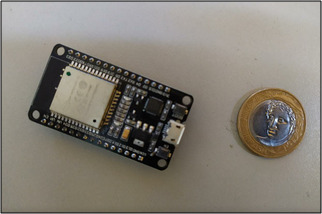
\includegraphics[height=5cm]{image2} \quad 
			\legend{Fonte: Própria}
			\caption{ERB ESP32}
			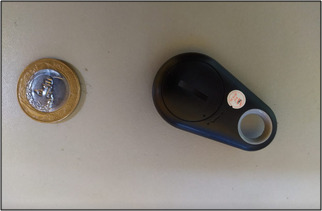
\includegraphics[height=5cm]{image3} 
			\legend{Fonte: Própria}	
		\end{center}
	\end{figure}	
\subsection{Programa}
Dividimos o projeto em duas partes, projeto de hardware e software, surgindo assim, dois programas fundamentais. Um programa definido para as ERBs e o outro para o visualizador web (software). As TAGs foram isoladas de programação devido às limitações do próprio fabricante dos beacon.
\subsubsection{Firmware}
	\begin{lstlisting}[style=myArduino]
/*  SENAI - PROJETO ESTAÇÃO SCANNER BLUETOOTH PARA LOCALIZAÇÃO INDOOR UTILIZANDO ESP32 */
//Biblioteca String para manipulação de variavel texto
#include <string>
//Biblioteca Wifi para gerenciamento de redes sem fio
#include <WiFi.h>
//Biblioteca PubSubClient para gerenciamento do protocolo MQTT
#include <PubSubClient.h>
//Bibliotecas BLE para gerenciamento do bluetooth
#include <BLEDevice.h>
#include <BLEUtils.h>
#include <BLEScan.h>
#include <BLEAdvertisedDevice.h>
//Constante que define a quantidade maxima que a estaçao poderá ler
#define MAX_BEACONS_BUFFER 50
//Constante que define o tempo de busca do bluetooth, em segundos
const int beaconScanTime = 4;
//Constante que o nome do dispositivo bluetooth da estação
const char *stationName = "Station 1";
//Constante que define o nome da rede WiFi
const char *ssid = "[YOUR_SSID]";
//Constante que define a senha da rede Wifi
const char *password = "[YOUR_PASSWORD]";
//Constante que define o nome do servidor Broker MQTT
const char *mqttServer = "[BROKER_HOST]";
//Constante que define a porta do Broker MQTT
const int mqttPort = [BROKER_PORT];
//Constante que define o usuário do Broker MQTT
const char *mqttUser = "[BROKER_USER]";
//Constante que define a senha do Broker MQTT
const char *mqttPassword = "[BROKER_PASS]";
//Constante que define os tópicos de subscrição para o MQTT
const char *subTopics[1] = {"/stations/command"};
//Constante que define os tópicos de publicação para o MQTT
const char *pubTopics[1] = {"/stations/beacons/get"};

//Estrutura de dados para armazenamento dos beacons
typedef struct
{
  //Endereço MAC do dispositivo bluetooth encontrado
  char address[17];
  //Potencia do sinal do dispositivo bluetooth encontrado
  int rssi;
  //Nome do dispositivo bluetooth encontrado
  char *bName;

} BeaconData; //Nome da estrutura de dados

//Objeto Wifi Client para gerenciamento da rede Sem fio
WiFiClient espClient;
//Objeto PubSubCliente para gerenciamento do protocolo MQTT
PubSubClient client(espClient);
//Array de Objetos que armazenara os dados dos beacons encontrados 
BeaconData beacons[MAX_BEACONS_BUFFER];
//Variavel para localização de um beacon dentro do array "beacons"
uint8_t beaconIndex = 0;
//Buffer para envio dos beacons no formato JSON
uint8_t message_char_buffer[MQTT_MAX_PACKET_SIZE];

//Classe personalizada que herda os métodos BLEAdvertisedDeviceCallbacks para subrecarga do método onResult
class MyAdvertisedDeviceCallbacks : public BLEAdvertisedDeviceCallbacks
{
public:
  //Sobrecarga do método onResult para tratamento dos dados recebidos pela busca bluetooth
  void onResult(BLEAdvertisedDevice advertisedDevice)
  {
    //Varivel relacionada a beaconIndex externa.
    extern uint8_t beaconIndex;
    //Varivel relacionada a beacons externo.
    extern BeaconData beacons[];

    //Valida a quantidade de beacons encontrados na busca
    if (beaconIndex >= MAX_BEACONS_BUFFER) return;
    //Valida a potencia de sinal do dispositivo encontrado
    if (advertisedDevice.haveRSSI()) beacons[beaconIndex].rssi = advertisedDevice.getRSSI();
    //Caso não possua sinal, é definido 0 para esse dispositivo
    else beacons[beaconIndex].rssi = 0;

    //Atribui o endereço MAC do dispositivo a variavel beacons[beaconIndex].address
    strcpy(beacons[beaconIndex].address, advertisedDevice.getAddress().toString().c_str());

    //Atribui o nome do dispositivo a variavel beacons[beaconIndex].bName
    std::string str = advertisedDevice.getName();
    beacons[beaconIndex].bName = new char[str.length() + 1];
    strcpy(beacons[beaconIndex].bName, str.c_str());
     
    //Incrementa mais um ao contador de dispositivos
    beaconIndex++;
  }
};
//Método de configuração do ESP
void setup()
{
  //Método de início a porta serial na velocidade 115200
  Serial.begin(115200);
  //Método de início ao dispositivo bluetooth 
  BLEDevice::init(stationName);
}
//Método de configuração WiFi
void connectWiFi()
{
  //Valida se o Wifi esta conectado a rede, caso nao esteja, inicia
  if (WiFi.status() != WL_CONNECTED) WiFi.begin(ssid, password);

  //Aguarda até que o status do wifi seja conectado
  while (WiFi.status() != WL_CONNECTED)
  {
    delay(2000);
    Serial.println("Connecting to WiFi...");
  }
}
//Método de configuração do protocolo MQTT
void connectMQTT()
{
  //Executa enquanto o protocolo está desconectado
  while (!client.connected())
  {
    //Define as credenciais do Broker MQTT
    client.setServer(mqttServer, mqttPort);
    //Define o método de callback para os tópicos de subscrição
    client.setCallback(mqttCallback);

    Serial.println("Connecting to MQTT...");
    //Tenta conexão e Valida se a conxão com o Broker funcionou
    if (client.connect("ESP32Client", mqttUser, mqttPassword))
    {
      Serial.println("Client Connected");
      Serial.println("Subscribing to topic:");
      boolean result;

      Serial.print(subTopics[0]);
      //Faz a subscrição no tópico definido em subTopics[0]
      result = client.subscribe(subTopics[0]);
      Serial.print(".....");
      Serial.println(result);
    }
    else
    {
      Serial.print("failed with state: ");
      Serial.print(client.state());
      delay(2000);
    }
  }
  //Coloca o protocolo MQTT em loop para novas mensagens
  client.loop();
}
//Método que escaneia os beacons e armazena os dados encontrados
void scanBeacons()
{
  delay(1000);
  //Objeto que define o scanner bluetooth
  BLEScan *pBLEScan = BLEDevice::getScan();
  //Objeto que define o método de callback
  MyAdvertisedDeviceCallbacks cb;
  //Configura o scanner para o callback definido
  pBLEScan->setAdvertisedDeviceCallbacks(&cb);
  //Configura o scanner como ativo
  pBLEScan->setActiveScan(true);
  //Objeto que receberá os dispositivos encontrados pelo scanner
  BLEScanResults foundDevices = pBLEScan->start(beaconScanTime);
  //Configura o scanner como inativo
  pBLEScan->stop();
  //Aguarda 1 segundo
  delay(1000);
}
//Método que trata as mensagens recebidas pelo protocolo MQTT
void mqttCallback(char *topic, byte *payload, unsigned int length)
{
  //Objeto para conversão da mensagem em String
  String strPayload = "";

  //Conversão da mensagem em String
  for (int i = 0; i < length; i++) strPayload += (char)payload[i];

  Serial.print("Message arrived in topic: ");
  Serial.print(topic);
  Serial.print(" => ");
  Serial.println(strPayload);

  //Validaçao da mensagem para comando de busca
  if (String(topic) == String(subTopics[0]) && strPayload == "find") scanBeacons();
  //Validaçao da mensagem para comando de envio de dados no formato CSV
  else if (String(topic) == String(subTopics[0]) && strPayload == "sendCSV") sendBeaconsCSV();
  //Validaçao da mensagem para comando de envio de dados no formato JSON
  else if (String(topic) == String(subTopics[0]) && strPayload == "sendJSON") sendBeaconsJSON();
  //Validaçao da mensagem para comando de busca e envio de dados no formato CSV
  else if (String(topic) == String(subTopics[0]) && strPayload == "findAndSendCSV") {
    //Busca os dispositivos
    scanBeacons();
    //Envia os dispositivos encontrados em formato CSV
    sendBeaconsCSV();
  }
  //Validaçao da mensagem para comando de busca e envio de dados no formato JSON
  else if (String(topic) == String(subTopics[0]) && strPayload == "findAndSendJSON")
  {
    //Busca os dispositivos
    scanBeacons();
    //Envia os dispositivos encontrados em formato JSON
    sendBeaconsJSON();
  }
}
//Método de envio das informações em formato JSON
void sendBeaconsJSON()
{
  //Varival de resultado da publicação no Broker MQTT
  boolean result;
  //Variavel de mensagem payload
  String payload = "{\"e\":[";

  for (uint8_t i = 0; i < beaconIndex; i++)
  {
    //Incremento do endereço
    payload += "{\"m\":\"";
    payload += String(beacons[i].address);
    //Incremento da força do sinal
    payload += "\",\"r\":\"";
    payload += String(beacons[i].rssi);
    //Incremento do nome
    payload += "\",\"n\":\"";
    payload += String(beacons[i].bName);
    payload += "\"}";
    if (i < beaconIndex - 1) payload += ',';
  }
  //Incremento do endereço da estação
  payload += "],\"stMac\":\"";
  payload += String(WiFi.macAddress());
  //Incremento do nome da estação
  payload += "\",\"stNome\":\"";
  payload += stationName;
  payload += "\"}";

  //Publicação da mensagem no Broker
  Serial.print("Publishing: ");
  Serial.print(payload);
  payload.getBytes(message_char_buffer, payload.length() + 1);
  result = client.publish_P(pubTopics[0], message_char_buffer, payload.length(), false);
  Serial.print(" -> Result: ");
  Serial.println(result);

  //Reseta a variavel para posição inicial
  beaconIndex = 0;
}
void sendBeaconsCSV()
{
  //Varival de resultado da publicação no Broker MQTT
  boolean result;
  for (uint8_t i = 0; i < beaconIndex; i++)
  {
    //Variavel de mensagem payload e Incremento do endereço da estação
    String payload = String(WiFi.macAddress());
    payload += ";";
    //Incremento do nome da estação
    payload += stationName;
    payload += ";";
    //Incremento do nome
    payload += String(beacons[i].bName);
    payload += ";";
    //Incremento do endereço
    payload += String(beacons[i].address);
    payload += ";";
    //Incremento da potencia do sinal
    payload += String(beacons[i].rssi);

    //Publicação da mensagem no Broker
    Serial.print("Publishing: ");
    Serial.print(payload);
    result = client.publish(pubTopics[0], (char *)payload.c_str());
    Serial.print(" -> Result: ");
    Serial.println(result);
  }
  //Reseta a variavel para posição inicial
  beaconIndex = 0;
}
void loop()
{
  //Método que valida a conexão do Wifi
  connectWiFi();
  //Método que valida a conexao com Broker MQTT
  connectMQTT();
  //Aguarda 0.5 segundos
  delay(500);
}
\end{lstlisting}
\subsubsection{Software}
Devido a complexidade do software ficará disponível o link para acesso ao conteúdo.
\newline
\begin{verbatim}
https://github.com/rafargp/Projeto_Senai
\end{verbatim}
\section{Validação}
\subsection{Testes}
Os primeiros testes foram feitos entre uma ERB utilizando uma placa ESP-32 e uma TAG utilizando um beacon, chegamos aos resultados mostrados na tabela 01
\begin{figure}[H]
	\begin{center}
		\caption{Intensidade de Sinal - BLE}
		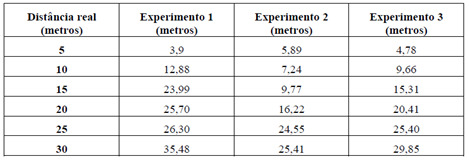
\includegraphics[height=5cm]{image7}
		\legend{Fonte: Própria}
	\end{center}
\end{figure}	
Através dos testes de distâncias foi possível desenvolver o programa para as ERBs. 
\subsection{Acertos}
A tabela foi transformada em uma tela de localização, onde houve o desenvolvimento de um software para localização. Utilizamos a programação web Hypertext Markup Language (HTML) conforme ilustrado na figura 02 para demonstrar de forma intuitiva a tela de lçocalização
\begin{figure}[H]
	\begin{center}
		\caption{Layout Software}
		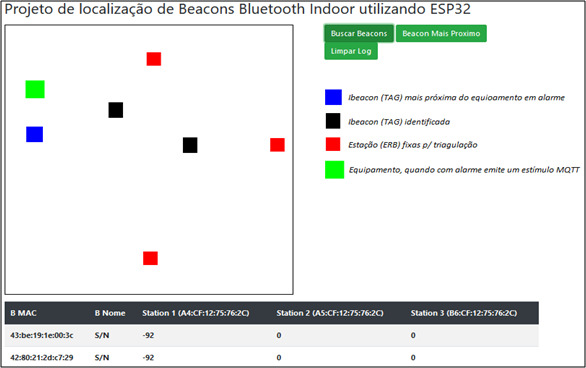
\includegraphics[height=5cm]{image4}
		\legend{Fonte: Própria}
	\end{center}
\end{figure}	
De acordo com a figura 05 o aplicativo para celular (APP) de alarmes foi modificado por uma programação na aplicação Node-RED da IBM para simulação das ERBs e equipamento com e sem alarmes.
\begin{figure}[H]
	\begin{center}
		\caption{Aplicação Node-Red}
		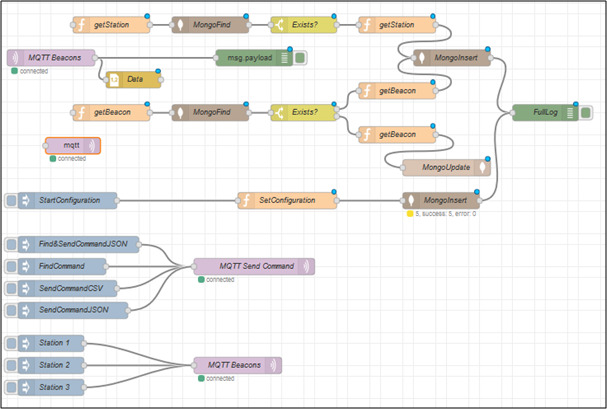
\includegraphics[height=5cm]{image5}
		\legend{Fonte: Própria}
	\end{center}
\end{figure}	
\section{Resultados}
Os resultados esperados foram alcançados, em destaque o software desenvolvido, onde é possível localizar pessoas em tempo real e monitorar a intensidade do sinal através da tabela de monitoramento conforme a figura 06.
\begin{figure}[H]
	\begin{center}
		\caption{Software de Monitoramento}
		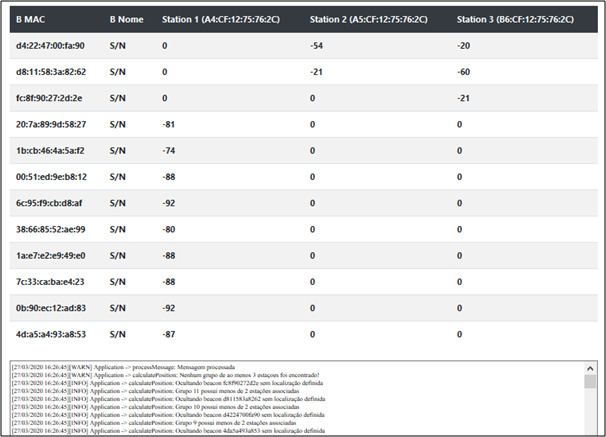
\includegraphics[height=5cm]{image6}
		\legend{Fonte: Própria}
	\end{center}
\end{figure}

\section{Conclusão}
Em vista que, foi possível demonstrar como funciona e como se monitora pessoas por sistema RSSI, pode se afirmar que foi alcançado o objetivo deste trabalho.
Os objetivos foram atingidos de forma, apresentado o principal tipo e modelo de localizador indoor e a sua utilização em sistema de missão crítica. Verificado o principal método de localização indoor, RSSI. Através dos ensaios e testes foi possível notar a importância de um bom programa (software) a manter um nível de confiabilidade de localização, através de algoritmos podendo corrigir erros causados por ruídos.
Para trabalhos futuros sugiro que analisem outros métodos de localização com tecnologia de rádio frequência e a viabilidade econômica em manter a localização indoor para grande alcance. Esse trabalho seria de grande valia também, pois demonstra a base do estudo de um sinal RFID, para avaliação da intensidade de sinal em um ambiente indoor.
Pode se concluir com este trabalho que através de ensaios e testes com componentes RSSI é possível garantir a localização de pessoas, diminuindo o risco de falhas e interrupções de funcionalidade em sistemas de missão crítica, garantindo um melhor aproveitamento dos técnicos que atuam para resolver problemas em data centers.

\section*{Agradecimentos}

Dedicamos este trabalho aos amigos e professores que nos apoiaram para nossa formação acadêmica.

%% \bibliographystyle{plain}
%% \bibliography{references.bib}
\section*{Referências}
PENSO, International Consortium for Organizational Resilience. Disponível em: https://www.penso.com.br/ . Acesso em: 16 mar. 2020.
\newline
ICOR, Infraestrutura de TI. Disponível em: https://www.build-resilience.org/ . Acesso em: 15 mar. 2020.
\newline
LIMA, Leonardo, Como a tecnologia pode ajudar na sua operação logística. Disponível em: http://www.cabtecgti.com.br/blog/ . Acesso em: 10 mar. 2020.
\newline
LIMA, E. A. (2001) Sistemas para Localização de Pessoas e Objetos em Ambientes
\newline
Indoor. Pontifícia Universidade Católica do Rio de Janeiro, Rio de Janeiro, RJ, Novembro.
\newline
OMEGA, Introdução aos sensores sem fio. Disponível em: https://br.omega.com/ . Acesso em: 16 mar. 2020.
\newline
LOUREIRO, A. A. F; NOGUEIRA, J. M. S; RUIZ, L. B; MINI, R. A. F; NAKAMURA, E. F; FIGUEIREDO, C. M. S. (2003) Redes de Sensores Sem Fio. . In: XXI Simpósio Brasileiro de Redes de Computadores (SBRC'03), Anais... Natal, RN, Brasil. Tutorial, p. 179-226.
\newline
ZHU, Q. et al. Iot gateway: Bridgingwireless sensor networks into internet of things. In:IEEE. Embedded and Ubiquitous Computing (EUC), 2010 IEEE/IFIP 8th InternationalConference on. [S.l.], 2010. p. 347–352.

\newpage
\textbf{Rafael Gomes de Paula} nasceu no Brasil, em 07 de julho de 1993. É formado em Técnico de Informatica pelo Colégio Cruzeiro do Sul em 2010 e em Ciência da Computação pela Universidade Cruzeiro do Sul em 2018. Ele trabalha na AXA Seguros do Brasil desde
2018, onde atualmente exerce a função de analista de sistemas.
Ele tem muito interesse em aplicações voltadas para o Agronegócio.
\newline
\newline\textbf{Wanderson Thiago da Silva Pagani} nasceu no Brasil, em 05 de abril de 1988. É formado em Eletrotécnica pela Escola SENAI "Antônio Devisate" em 2004, em Engenharia Elétrica pela Universidade Anhanguera - CL em 2019 e atualmente cursando Pós-graduação na Escola SENAI "Mariano Ferraz". Ele trabalha na PRODESP Companhia de Processamento de Dados do Estado de São Paulo desde
2013, onde atualmente exerce a função de Supervisor de Manutenção no Sistema de Missão Crítica.
Ele tem muito interesse em aplicações voltadas para data centers.
\newline
\newline\textbf{Josimar de Andrade Silva}, nascido em São Paulo em 14 de dezembro de 1986. Técnico em Eletroeletrônica formado no Senai “Roberto Simonsen ” em 2003 e Engenharia de Controle e Automação pela Universidade Anhanguera em 2012. Atualmente desempregado e em busca de novas oportunidades, vinha atuando na Hyundai Rotem, empresa coreana fabricante de uma das novas frotas de trens de São Paulo, realizando o comissionamento estático e dinâmico dos trens buscando a validação de segurança e desempenho, para que os mesmos possam entrar em operação nas linhas da CPTM.
\end{document}